\chapter{Hồi quy phi tham số và các mở rộng}\label{ch:regression}
\section{Mục tiêu hồi quy khác mục tiêu mật độ}
Quan sát các cặp i.i.d. $(X_i,Y_i)$, mô hình
\[
Y_i=r(X_i)+\varepsilon_i,\qquad
\E(\varepsilon_i\mid X_i)=0,\qquad
\Var(\varepsilon_i\mid X_i)=\sigma^2(X_i).
\]
Ta ước lượng $r(x)=\E(Y\mid X=x)$.
Ký hiệu $f(x)$ trong chương này là mật độ của \emph{biến thiết kế} $X$,
không phải hàm hồi quy. Hàm $r$ không cần không âm hay tích phân bằng 1.
Giả thiết kỳ vọng có điều kiện bằng 0 là điều cần để nhận $r$ là hàm
hồi quy; chỉ $\E\varepsilon=0$ chưa đủ.
\intuition{KDE hỏi ``dữ liệu $X$ tập trung ở đâu?''; hồi quy hỏi
``tại giá trị $X=x$, trung bình $Y$ là bao nhiêu?''. Cùng kernel nhưng
khác đối tượng cần ước lượng.}

\section{Nadaraya--Watson từ bình phương tối thiểu cục bộ}
Với $k_i(x)=K((X_i-x)/h)$, $K\geq0$, xấp xỉ $r$ gần $x$ bằng hằng
$a$ và giải $Q(a)=\sum_i k_i(Y_i-a)^2$.
\[
Q'(a)=-2\sum_i k_iY_i+2a\sum_i k_i=0.
\]
Nếu $\sum_i k_i>0$, $Q''(a)=2\sum_i k_i>0$ nên nghiệm duy nhất:
\[
\boxed{\widehat r_{\rm NW}(x)=\frac{\sum_i k_iY_i}{\sum_i k_i}
=\sum_i w_iY_i,\qquad w_i=\frac{k_i}{\sum_jk_j}.}
\]
Trọng số không âm, tổng 1, nên dự đoán nằm giữa các $Y_i$ có trọng số.
Nếu dùng $K((x-X_i)/h)$, cùng công thức cho kernel đối xứng.
Nhân compact có thể cho mẫu số 0 khi không có điểm trong cửa sổ;
estimator khi đó không xác định, không gán 0 tùy ý.

\begin{example}
$X=(1,2,4,5)$, $Y=(2,3,7,8)$, $x=3,h=2$, Epanechnikov cho
$k=(0,9/16,9/16,0)$. Vì thế
\[
\widehat r_{\rm NW}(3)=\frac{(9/16)3+(9/16)7}{9/16+9/16}=5.
\]
Trong bài KDE với cùng $X$, kết quả mật độ là $9/64$, một đại lượng khác.
\end{example}

\subsection{Từ tỷ số mật độ đến công thức NW}
Nếu $(X,Y)$ có mật độ đồng thời $p(x,y)$ và $f(x)>0$,
$r(x)=\int yp(x,y)dy/f(x)$.
Dùng nhân tích cho mật độ đồng thời,
\[
\widehat p(x,y)=\frac1{nhb}\sum_iK((x-X_i)/h)L((y-Y_i)/b).
\]
Giả sử $\int L=1$, $\int vL(v)dv=0$, moment tuyệt đối bậc nhất hữu hạn.
Đặt $v=(y-Y_i)/b$:
\[
\int y\frac1bL((y-Y_i)/b)\,dy
=\int(Y_i+bv)L(v)\,dv=Y_i.
\]
Tích phân theo $y$ cho mật độ biên
$(nh)^{-1}\sum_iK((x-X_i)/h)$; tích phân có thừa số $y$ cho
$(nh)^{-1}\sum_iK((x-X_i)/h)Y_i$. Tỷ số triệt tiêu $1/(nh)$, chính
là NW. Mối liên hệ này không yêu cầu mọi bài hồi quy đều có mật độ
đồng thời; phép suy ra từ bình phương tối thiểu vẫn dùng được khi $Y$ rời rạc.
\intuition{NW là trung bình có trọng số của các đáp ứng gần $x$.
Ở nơi mật độ thiết kế cao hơn, có nhiều quan sát hơn kéo trung bình về phía đó.}
\source{\cite{wasserman}, Mục 5.4.1, trang in 72--73 (PDF 82--83);
\cite{tsybakov}, Mục 1.5}

\section{Design bias: thành phần phụ thuộc mật độ thiết kế}
Xét mục tiêu làm trơn ở mức quần thể
\[
r_h(x)=\frac{\int K(u)r(x+hu)f(x+hu)du}
{\int K(u)f(x+hu)du}.
\]
Đây là tỷ số các kỳ vọng, không phải đẳng thức chính xác với
$\E\widehat r_{\rm NW}(x)$ ở mẫu hữu hạn.
Giả sử $x$ là điểm nội, $f(x)>0$, $f,r$ có hai đạo hàm liên tục và
kernel chẵn có moment bậc hai. Đặt $g=rf$, $c=h^2\mu_2(K)/2$:
\[
\int K(u)g(x+hu)du=g(x)+cg''(x)+o(h^2),\quad
\int K(u)f(x+hu)du=f(x)+cf''(x)+o(h^2).
\]
Vì $1/(f+c f''+o(h^2))=f^{-1}-cf''f^{-2}+o(h^2)$,
\begin{align*}
r_h(x)&=r(x)+c\left[\frac{(rf)''}{f}-\frac{r f''}{f}\right]+o(h^2)\\
&=r(x)+c\left[r''(x)+2\frac{r'(x)f'(x)}{f(x)}\right]+o(h^2),
\end{align*}
vì $(rf)''=r''f+2r'f'+rf''$; hai hạng $rf''/f$ triệt tiêu.
Vậy bias làm trơn dẫn đầu là
\[
\boxed{r_h(x)-r(x)=\frac{h^2\mu_2(K)}2
\left[r''(x)+2\frac{r'(x)f'(x)}{f(x)}\right]+o(h^2).}
\]
Phần $2r'f'/f$ được gọi là \emph{design bias}.
Nếu $r$ tuyến tính, $r''=0$ nhưng $r'f'\ne0$, NW vẫn chệch.
Với $r(x)=x$, $f(x)=2x$ tại $x=1/2$, thành phần trong ngoặc bằng 4.

Để chuyển sang phát biểu tiệm cận cho estimator ngẫu nhiên cần kiểm soát
tỷ số và dao động của các moment thiết kế. Với kernel compact bị chặn,
mật độ thiết kế dương, trơn và $nh^3\to\infty$, sai số moment bậc một
do mẫu có bậc $O_P(h/\sqrt{nh})=o_P(h^2)$, nên bias có điều kiện
theo thiết kế cũng có khai triển trên ở điểm nội.
Phương sai do nhiễu có dạng chính
\[
\Var(\widehat r_{\rm NW}(x)\mid X_1,\ldots,X_n)
\approx\frac{\sigma^2(x)R(K)}{nhf(x)}.
\]
Không nhầm với variance KDE $f(x)R(K)/(nh)$:
trong hồi quy, mật độ thiết kế nhỏ làm ít dữ liệu hữu hiệu và tăng variance.
\intuition{NW dùng một hằng số để xấp xỉ đoạn có độ dốc. Khi các điểm
không cân đối hai phía, hằng số bị kéo về phía đông dữ liệu.}

\section{Local linear: hệ phương trình và trọng số}
Thay hằng số bằng đường thẳng cục bộ, $d_i=X_i-x$:
\[
\min_{a_0,a_1}\sum_i k_i[Y_i-a_0-a_1d_i]^2.
\]
Đặt $S_q=\sum_i k_id_i^q$, $T_q=\sum_i k_id_i^qY_i$.
Đạo hàm theo hai hệ số cho hệ phương trình chuẩn
\[
\begin{pmatrix}S_0&S_1\\S_1&S_2\end{pmatrix}
\begin{pmatrix}\widehat a_0\\\widehat a_1\end{pmatrix}
=\begin{pmatrix}T_0\\T_1\end{pmatrix}.
\]
Nếu $\Delta=S_0S_2-S_1^2>0$, nghịch đảo ma trận cho
\[
\boxed{\widehat r_{\rm LL}(x)=\widehat a_0
=\frac{S_2T_0-S_1T_1}{\Delta}
=\sum_iw_i^{\rm LL}Y_i,\quad
w_i^{\rm LL}=\frac{k_i(S_2-S_1d_i)}\Delta.}
\]
Với $S_0>0$, $\Delta/S_0^2$ là phương sai có trọng số của các $d_i$.
Do đó $\Delta>0$ khi có ít nhất hai vị trí $X_i$ khác nhau với trọng số
dương. Nếu chỉ một vị trí, đường thẳng không xác định duy nhất.

Hai đẳng thức then chốt:
\[
\sum_iw_i^{\rm LL}=\frac{S_2S_0-S_1^2}\Delta=1,\qquad
\sum_iw_i^{\rm LL}d_i=\frac{S_2S_1-S_1S_2}\Delta=0.
\]
Trọng số có thể âm nhưng tổng vẫn 1. Nếu $Y_i=a+bX_i$, khi $\Delta>0$,
\[
\widehat r_{\rm LL}(x)=\sum_iw_i[a+bx+bd_i]=a+bx,
\]
nên local linear tái tạo chính xác mọi hàm tuyến tính, kể cả gần biên.
\intuition{Trọng số local linear tự điều chỉnh để moment bậc một bằng 0.
Không cần dữ liệu hai phía cân đối để triệt tiêu ảnh hưởng của độ dốc.}
\source{\cite{wasserman}, Mục 5.4.2; \cite{tsybakov}, Mục 1.6,
Mệnh đề 1.12, trang in 36 (PDF 47)}

\section{Vì sao local linear giảm design bias và chệch biên?}
\subsection{Chứng minh trực tiếp bằng tái tạo tuyến tính}
Lấy kỳ vọng có điều kiện theo các $X_i$ và khai triển $r$:
\begin{align*}
\E(\widehat r_{\rm LL}(x)\mid X)
&=\sum_iw_i[r(x)+r'(x)d_i+\tfrac12r''(x)d_i^2+o(d_i^2)]\\
&=r(x)+\tfrac12r''(x)\sum_iw_id_i^2+
\sum_iw_io(d_i^2).
\end{align*}
Hằng số giữ nguyên do tổng trọng số bằng 1; hạng bậc nhất mất do tổng
$w_id_i$ bằng 0. Không xuất hiện phần $r'f'/f$.
Với kernel compact, $|d_i|\leq h$ khi $k_i>0$.
Nếu ma trận moment không suy biến và $\sum_i|w_i|$ bị chặn,
\[
|\E(\widehat r_{\rm LL}(x)\mid X)-r(x)|
\leq\tfrac12\norm{r''}_\infty h^2\sum_i|w_i|=O(h^2).
\]
Điều này áp dụng cả ở biên khi moment một phía vẫn không suy biến.
``Giảm boundary bias'' nghĩa là bỏ chệch bậc nhất, không phải bias bằng 0.
Các giả thiết thiết kế dương trên miền, độ trơn và kiểm soát nghịch đảo
ma trận là cần thiết; không tuyên bố $O(h^2)$ ở điểm không có dữ liệu.

\subsection{Hằng số tại điểm nội và tại biên}
Ở điểm nội, moment thiết kế có dạng
$S_q/(nh^{q+1})\to f(x)\mu_q(K)$. Với kernel chẵn,
$\mu_1=0$, nên
\[
\sum_iw_id_i^2=\frac{S_2^2-S_1S_3}{\Delta}
=h^2\mu_2(K)+o_P(h^2).
\]
Bias chính là $h^2\mu_2r''/2$, không có design bias bậc hai.
Tại biên trái $x=0$ trên $[0,1]$, dùng moment một phía
$m_q=\int_0^1u^qK(u)du$ cho kernel compact:
\[
\sum_iw_id_i^2\approx
h^2\frac{m_2^2-m_1m_3}{m_0m_2-m_1^2}.
\]
Với Uniform, $(m_0,m_1,m_2,m_3)=(1/2,1/4,1/6,1/8)$,
tỷ số bằng $-1/6$, nên bias tại 0 là $-h^2r''(0)/12$.
NW tại 0 có bias làm trơn $hr'(0)/2+O(h^2)$.
Kernel tương đương của local linear tại biên là $4-6u$ trên $[0,1]$,
cùng cấu trúc moment với boundary kernel ở Chương 3.

\subsection{Phương sai và điều kiện sử dụng}
Với nhiễu độc lập có điều kiện theo thiết kế,
\[
\Var(\widehat r_{\rm LL}(x)\mid X)=\sum_iw_i^2\sigma^2(X_i).
\]
Nếu $\max_i|w_i|=O(1/(nh))$, $\sum_i|w_i|=O(1)$ và variance nhiễu
bị chặn, variance là $O(1/(nh))$.
Ở điểm nội có hằng số chính $\sigma^2(x)R(K)/(nhf(x))$ với kernel
đối xứng chuẩn hóa. Ở biên, thay $R(K)$ bằng bình phương tích phân của
kernel tương đương; hằng số thường lớn hơn.
Trọng số âm giúp sửa bias nhưng có thể làm dự đoán ra ngoài khoảng các
$Y_i$ lân cận. Nếu ma trận gần suy biến, cần mở rộng bandwidth hoặc
báo thiếu hỗ trợ thiết kế, không nghịch đảo máy móc.

\begin{figure}[htbp]
\centering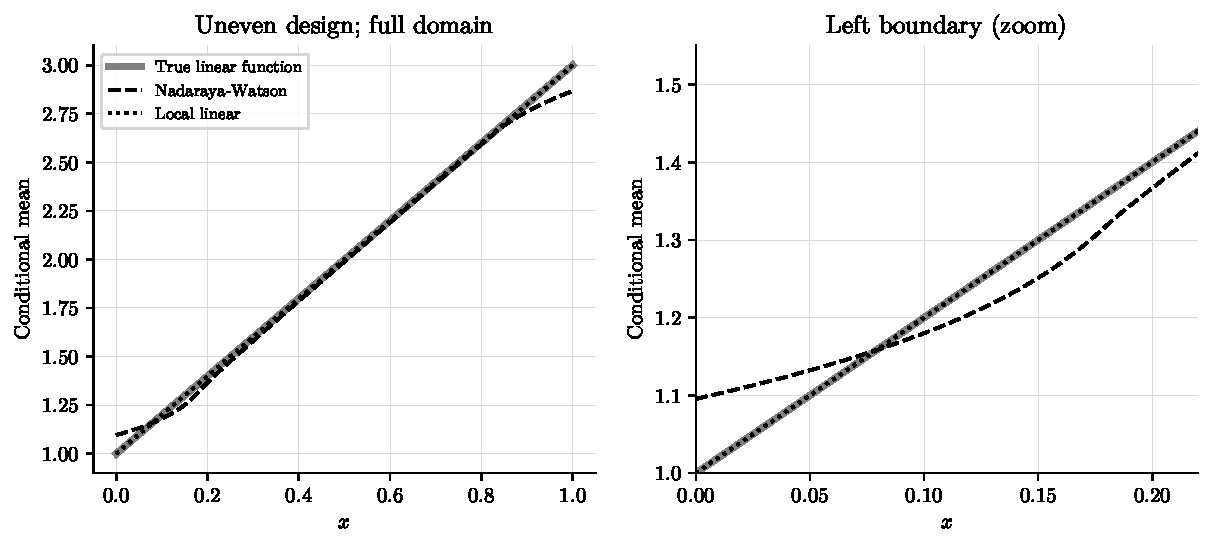
\includegraphics[width=.95\textwidth]{regression.pdf}
\caption{Làm trơn hàm tuyến tính trên các điểm thiết kế không đều,
$h=0.18$, kernel Epanechnikov. Đường vẽ dùng $Y_i=r(X_i)$ không có
nhiễu, nên biểu diễn kỳ vọng có điều kiện. Local linear tái tạo đường
thẳng; NW bị kéo bởi thiết kế và gần biên.}
\end{figure}
\intuition{Local linear dùng độ dốc như một tham số phụ để ước lượng
giá trị tại tâm chính xác hơn. Độ dốc không cần phải được báo cáo để
phương pháp tận dụng được nó.}

\section{Root--Unroot: từ số đếm đến hồi quy}
\subsection{Binning và xấp xỉ Poisson}
Giả sử mật độ trên $[0,1]$. Chia $k$ ô bằng nhau, trung điểm
$t_j=(j-1/2)/k$, số đếm $N_j$, xác suất ô $p_j$.
Nếu $f$ ít biến thiên trong ô,
$p_j\approx f(t_j)/k$ và $\lambda_j=np_j\approx nf(t_j)/k$.
Trong mô hình cố định $n$, $(N_1,\ldots,N_k)$ đa thức,
\[
\E N_j=np_j,\quad\Var N_j=np_j(1-p_j),\quad
\Cov(N_j,N_\ell)=-np_jp_\ell\quad(j\ne\ell).
\]
Các số đếm không độc lập. Với ô có xác suất nhỏ, từng số đếm có thể
xấp xỉ Poisson; trong mô hình Poisson hóa tổng số quan sát,
các số đếm độc lập Poisson thật sự.

\subsection{Lấy căn để ổn định phương sai}
Với $N\sim\operatorname{Poisson}(\lambda)$, xét $g(N)=\sqrt{N+c}$.
Delta method cho
\[
\Var g(N)\approx[g'(\lambda)]^2\lambda
=\frac{\lambda}{4(\lambda+c)}\approx\frac14
\]
khi $\lambda$ lớn. Taylor bậc hai cho kỳ vọng:
\begin{align*}
\E g(N)&\approx\sqrt{\lambda+c}
-\frac{\lambda}{8(\lambda+c)^{3/2}}\\
&=\sqrt\lambda+\frac{c/2-1/8}{\sqrt\lambda}
+\text{các hạng bậc nhỏ hơn}.
\end{align*}
Chọn $c=1/4$ triệt tiêu hiệu chỉnh bias dẫn đầu.
Đây là xấp xỉ, không phải kỳ vọng chính xác của căn số đếm.
Đặt
\[
\boxed{Y_j=\sqrt{\frac{k}{n}(N_j+1/4)}.}
\]
Khi xấp xỉ đủ tốt,
\[
Y_j\approx r(t_j)+\sigma\varepsilon_j,
\quad r(x)=\sqrt{f(x)},\quad \sigma^2\approx\frac{k}{4n},
\quad\varepsilon_j\text{ gần chuẩn tắc}.
\]
Ở ô rất ít số đếm, gần chuẩn có thể kém. Quy tắc $k\approx n/10$ trong
Wasserman là lựa chọn thực hành, không bảo đảm điều kiện tiệm cận hay
đếm đủ lớn ở mọi ô.

\subsection{Hồi quy, lấy phần dương và chuyển ngược}
Áp dụng hồi quy phi tham số cho $(t_j,Y_j)$ để có $\widehat r(x)$.
Đặt $r_+(x)=\max\{\widehat r(x),0\}$ và
\[
\boxed{\widehat f_{\rm RU}(x)=
\frac{r_+(x)^2}{\int_0^1r_+(t)^2\,dt}.}
\]
Phải kiểm tra mẫu số hữu hạn và dương. Nếu mẫu số bằng 0, quy trình
không trả được mật độ, cần xem lại hồi quy hoặc dữ liệu.
Lấy phần dương trước bình phương tránh biến một dự đoán âm của căn mật
độ thành mật độ lớn giả tạo. Chuẩn hóa đảm bảo tổng diện tích 1.

\begin{example}
$n=40$, $k=4$, số đếm $(4,8,12,16)$, nên
\[
Y_j^2=(N_j+1/4)/10=(0.425,0.825,1.225,1.625).
\]
$\sigma^2\approx0.025$, $\sigma\approx0.15811$.
Nếu \emph{chưa làm trơn} và giữ căn hằng theo từng ô, tích phân bình
phương là $(0.425+0.825+1.225+1.625)/4=1.025$.
Chiều cao chuẩn hóa là $(17,33,49,65)/41$.
Ví dụ chỉ kiểm tra biến đổi và chuẩn hóa; bước hồi quy thực sự vẫn cần
thiết lập bandwidth hoặc mức mô hình riêng.
\end{example}
\intuition{Binning tạo dữ liệu hồi quy; bước hồi quy mới quyết định độ
trơn cuối cùng. Lấy căn làm nhiễu ở các ô có mật độ khác nhau gần cùng
variance, rồi unroot đưa kết quả về mật độ.}
\source{\cite{wasserman}, Mục 6.6, trang in 139--140 (PDF 148--149)}

\section{Root--Unroot và băng tin cậy: mục tiêu nào được phủ?}
Trong mô hình Gaussian hồi quy lý tưởng, một smoother tuyến tính
$\widehat r(x)=\sum_j\ell_j(x)Y_j$ có kỳ vọng
$r_s(x)=\sum_j\ell_j(x)r(t_j)$ và variance
$\sigma^2\sum_j\ell_j(x)^2$ nếu các nhiễu độc lập.
Trên lưới $q$ điểm $x_1,\ldots,x_q$, khi $\sigma$ biết và mô hình đúng,
Bonferroni cho khoảng đồng thời của $r_s$ trên lưới:
\[
\widehat r(x_a)\pm z_{1-\alpha/(2q)}\sigma
\sqrt{\sum_j\ell_j(x_a)^2},\quad a=1,\ldots,q.
\]
Vì tổng xác suất thất bại ở $q$ điểm không quá $\alpha$, các khoảng
phủ đồng thời ít nhất $1-\alpha$. Đây chưa phải băng trên continuum;
mô hình Root--Unroot thật còn có sai số Poisson/Gaussian và binning.
Muốn phủ $r=\sqrt f$ thay vì $r_s$, phải xử lý bias hoặc undersmooth.

Giả sử đã có băng hợp lệ $L(x)\leq\sqrt{f(x)}\leq U(x)$ trên cả miền.
Vì hàm bình phương đơn điệu trên $[0,\infty)$,
\[
[\max\{L(x),0\}]^2\leq f(x)\leq[\max\{U(x),0\}]^2
\]
trên sự kiện phủ. Không tự chuẩn hóa hai đầu băng bằng cùng mẫu số
ngẫu nhiên của estimator: điều đó đổi đối tượng phủ và cần chứng minh
riêng. Chỉ bình phương khoảng cho $r_s$ cho khoảng của $r_s^2$, không
nhất thiết của mật độ thật $f$.
\intuition{Một biến đổi đẹp không xóa chệch làm trơn hay sự phụ thuộc của
số đếm. Cần báo rõ băng phủ hàm thật, hàm đã làm trơn, hay chỉ các giá trị
trên một lưới.}
\source{\cite{wasserman}, Mục 5.7, đặc biệt trang in 89--90 (PDF 99--100),
và Mục 6.6}

\section{KDE nhiều chiều và lời nguyền số chiều}
Với $X_i\in\R^d$, kernel tích chuẩn hóa và bandwidth chung $h$,
\[
\widehat f_h(x)=\frac1{nh^d}\sum_i
\prod_{a=1}^dK((x_a-X_{ia})/h).
\]
Đổi biến từng tọa độ cho $dx=h^ddu$, nên tích phân estimator bằng 1.
Với kernel đối xứng bậc hai, mật độ đủ trơn, miền không gây bias biên,
Taylor nhiều chiều cho
\[
\Bias(\widehat f_h(x))=
\frac{h^2\mu_2(K)}2\sum_{a=1}^d\partial_{aa}f(x)+o(h^2),
\quad
\Var\widehat f_h(x)\approx\frac{f(x)R(K)^d}{nh^d}.
\]
Hạng bậc một mất do moment một bằng 0. Hạng hỗn hợp
$u_au_b$ với $a\ne b$ mất vì tích hai moment một; hạng đường chéo
$u_a^2$ giữ lại, cho Laplacian $\sum_a\partial_{aa}f$.
Với phần dư tích phân kiểm soát được, AMISE có dạng
$Ah^4+B/(nh^d)$. Đạo hàm:
\[
4Ah^3-\frac{dB}{nh^{d+1}}=0
\quad\Longrightarrow\quad
\boxed{h_*\asymp n^{-1/(4+d)},\quad\MISE=O(n^{-4/(4+d)}).}
\]
Ở $d=1$, số mũ $4/5$; $d=6$, số mũ chỉ còn $2/5$.
Giả sử bỏ qua hằng số và muốn cùng quy mô sai số như $d=1$, cỡ mẫu
$n_1$, cần $n_d\approx n_1^{(d+4)/5}$.
Nếu $n_1=100$, thì $n_2\approx251$, $n_6\approx10\,000$,
$n_{10}\approx398\,107$. Đây chỉ là so sánh theo tốc độ, không phải
cỡ mẫu bảo đảm cho mọi mật độ.
\intuition{Thể tích cửa sổ giảm theo $h^d$, nên dữ liệu lân cận nhanh
chóng thưa khi tăng số chiều. Cấu trúc bổ sung như mô hình cộng hoặc
chiều nội tại thấp có thể giúp, nhưng thay đổi lớp bài toán và giả thiết.}
\source{\cite{wasserman}, Mục 6.5, trang in 138--139 (PDF 147--148)}
